\subsection{Phishing}
\label{sub:phishing}

Das Bestreben, persönliche Daten im Internet durch ein gezielt verfälschtes
Auftreten abzugreifen wird als Phishing (aus dem Englischen \emph{fishing}, für
\emph{fischen} oder \emph{angeln}) bezeichnet. In der Regel handelt es sich
dabei um E-Mail-Nachrichten oder Webseiten, welche Informationen wie Name,
Adresse, Benutzername/Passwort oder Kreditkarten-Daten anfordern. Dem Empfänger
wird dargelegt, sein Account auf einer Webseite würde in Gefahr sein, sollten
die geforderten Informationen nicht rasch übergeben werden. Dieses künstliches
Drängen soll den Adressaten der Phishing-Nachricht davon abhalten, seinen
Verstand zu benutzen und stattdessen eine panische, reflexartige Handlung
auslösen. Diese Handlung wird vom Betrüger geschickt dirigiert: dem Opfer wird
ein großer Button oder ein einfach erreichbarer Link präsentiert, der auf die
Webseite des Betrügers führt. Diese Webseite imitiert das Aussehen des
Originals, leitet jedoch die vom Benutzer eingetragenen Daten an den Sender der
Phishing-Nachricht weiter.

\begin{figure}
  \centering
  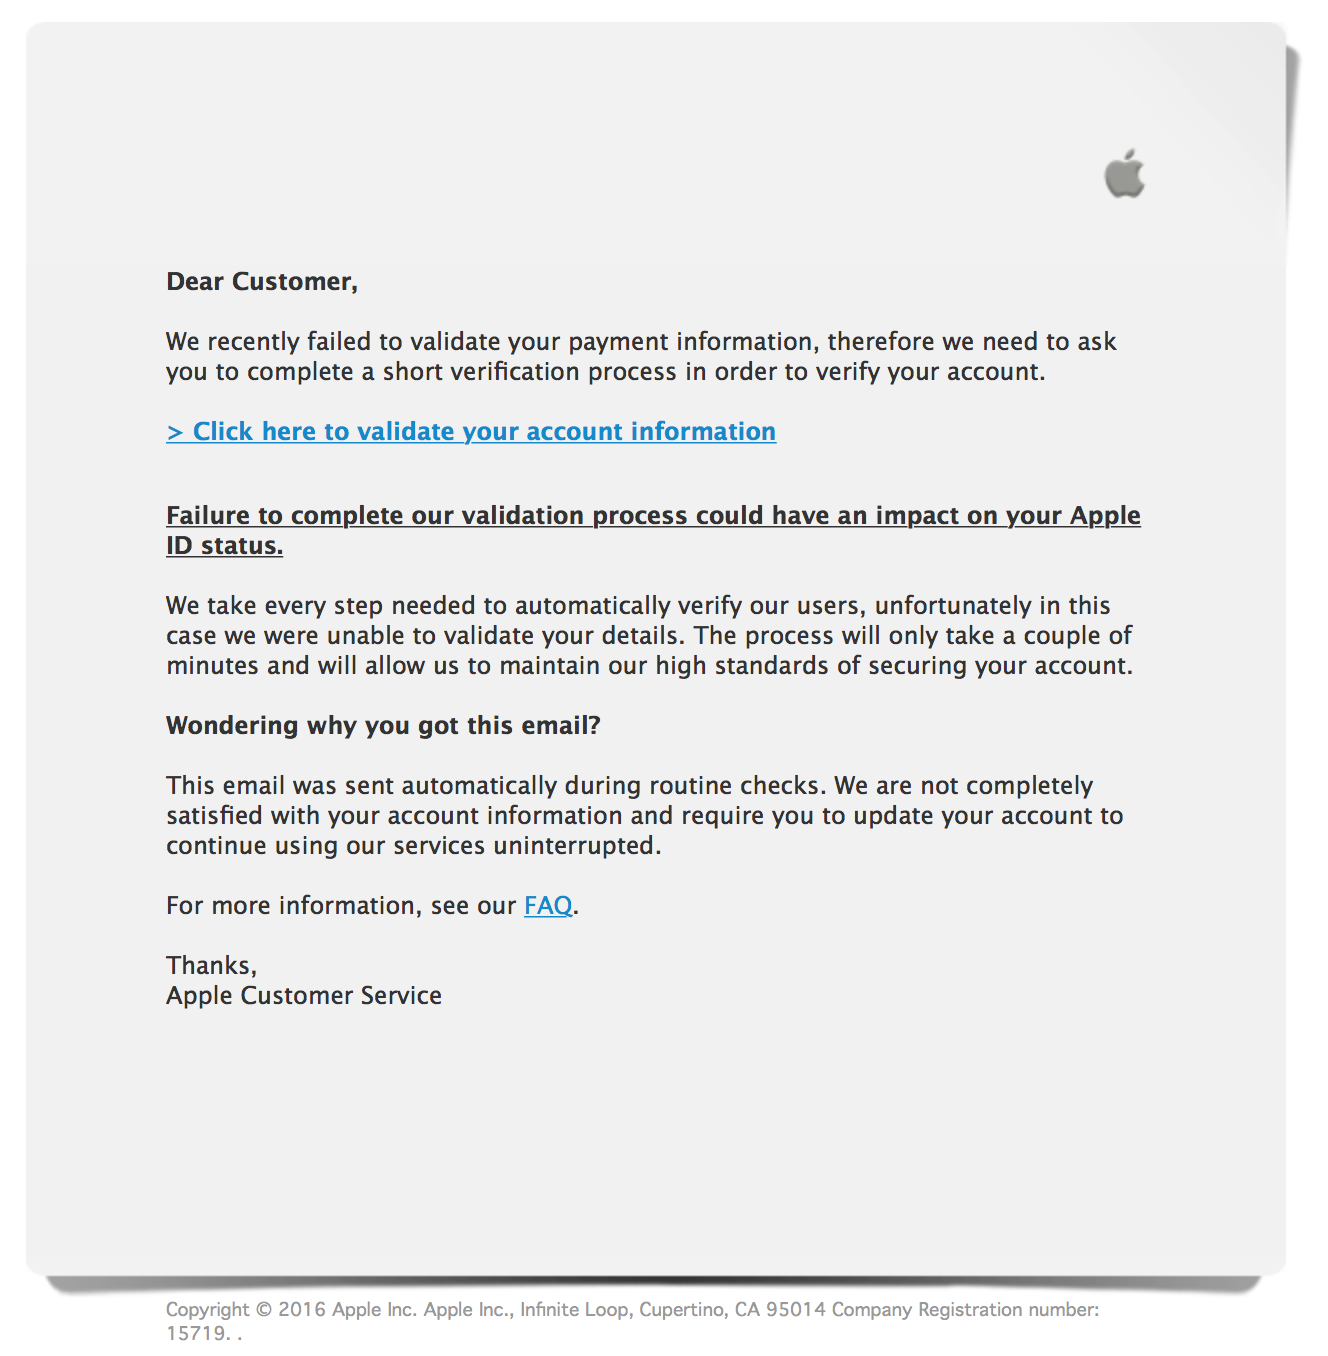
\includegraphics[scale=0.5]{Resources/phishing-apple}
  \caption{Eine Phishing-E-Mail, die das Aussehen einer E-Mail der Firma Apple Inc. imitiert}
  \label{fig:phishing-apple}
\end{figure}

Phishing ist eine besonders elegante Art des Spams, da die Opfer häufig nicht
mitbekommen, dass ihre Daten von Dritten abgegriffen werden. Nachdem man die
geforderten Daten eingegeben und abgesendet hat, leitet die Webseite des
Betrügers das Opfer auf die tatsächliche Webseite weiter.

Der Link \emph{> Click here to validate your account information} in der
Abbildung \ref{fig:phishing-apple} führt nicht auf die Domäne
\texttt{apple.com}. Der Quellcode der abgebildeten E-Mail und Bildschirmfotos
der verlinkten Webseite finden sich unter
\url{https://github.com/SoftwareAgenten/GA-Archive/tree/master/Phishing%20Mails/Apple\%20ID}.
